\documentclass[12pt]{jsarticle}
\usepackage{geometry}
\geometry{left=10mm,right=10mm,top=3mm,bottom=15mm}		
\usepackage{amssymb}
\usepackage{mathcomp}
\usepackage{amsmath,amsthm} 
\usepackage[dvipdfmx]{graphicx}
\usepackage{txfonts}
\usepackage[dvipdfmx]{hyperref}
\usepackage{pxjahyper}
\newenvironment{solution}
  {\renewcommand\qedsymbol{$\blacksquare$}\begin{proof}[Solution]}
  {\end{proof}}
\begin{titlepage}
\title{\Huge{空気力学第二D レポート}}
\author{\LARGE{工学部航空宇宙工学科三年 野本陽平 (03-180332)}}
\date{\large{提出日: 2019年2月1日}}
\thispagestyle{empty}
\end{titlepage}
\begin{document}
\maketitle
\section*{課題}
各自, 適当な対象を設定し, 計算機でシミュレーションしてみた結果をA4用紙2, 3枚程度にまとめて報告せよ. その際に問題設定, 使用した計算機・OS・プログラミング言語など, 解法, 結果の図(グラフィックス), 結果から自分が発見したこと などを明記すること.
\section{問題設定}
角柱(1本, 2本, 3本)及び近似された円柱周りの非圧縮流れを計算機を用いてシミュレーションした. 角柱は正方形断面である. 計算領域は$D=\{(x,y)|-10\le x\le 30, -10\le y\le 10\}$であり, 空間刻みは$dx=0.1, dy=0.1$とし, $x$方向$401$と$y$方向$201$の計$80601$のマトリックスで空間を定義した. クーラン数は$C=0.2$で, 時間刻みは$dt=C\times min(dx, dy)=0.02$. レイノルズ数は$Re=70$(角柱の場合), $Re=184000$(円柱の場合). $D$の境界では$p$は$0$とし, 全域で$u=1.0$(角柱の場合), $u=0.7$(円柱の場合)とした. 角柱の場合はスタンダードな環境での計算を解くためにこの条件にし(これは課題の要求を満たす箇所である), 円柱の場合はシステム学実験での水槽の実験と比較するために当時のレポートで記入したレイノルズ数等の条件を用いた. すなわち本レポートはシステム学実験において実際に行った実験と数値計算解を比較したレポートである.
\section{使用した計算機, OS, プログラミング言語など}
愛用の2016版mac book proを用いた. 可視化には慣れているpythonモジュールのmatplotlib.pyplotを用い, 計算には高速化が容易なC++を用いた. 以下は詳細である.
\begin{table}[htb]
  \begin{center}
    \begin{tabular}{|c|c|} \hline
      CPU(プロセッサ) & 2 GHz Intel Core i5 \\
      メモリ & 8 GB 1867 MHz LPDDR3 \\
      OS & macOS Mojave ver 10.14 \\
      使用言語 & C++17 \\
      コンパイラ & GNU GCC g++ \\  \hline
    \end{tabular}
  \end{center}
\caption{使用機器・ソフトウェア詳細}
\end{table}
\section{解法・結果の図(グラフィックス)}
圧力場の解析にはPoisson方程式をGauss-Seidel法を用いて解く. 速度場の解析にはKawamuraスキームを用いて解く. 以下ではレポート枚数制限の都合上圧力場のみを記載する. コードの詳細は \url{https://github.com/yohei-freelance/karman_vortex} 参照.
\begin{figure}[htbp]
 \begin{minipage}{0.5\hsize}
  \begin{center}
   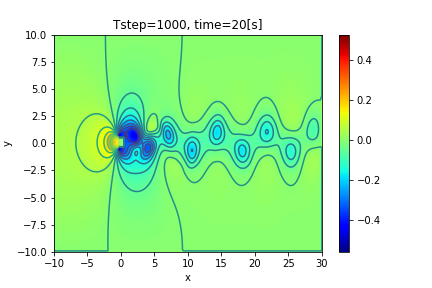
\includegraphics[width=65mm]{object_1.png}
   \caption{$Re=70, u=1.0[m/s]$のとき(角柱1本)}
  \end{center}
  \label{fig:one}
 \end{minipage}
 \begin{minipage}{0.5\hsize}
  \begin{center}
   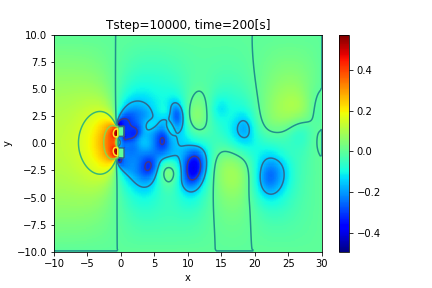
\includegraphics[width=65mm]{object_4.png}
   \caption{$Re=70, u=1.0[m/s]$のとき(角柱2本; 段差なし)}   
  \end{center}
  \label{fig:two}
 \end{minipage}
\end{figure}
\begin{figure}[htbp]
 \begin{minipage}{0.5\hsize}
  \begin{center}
   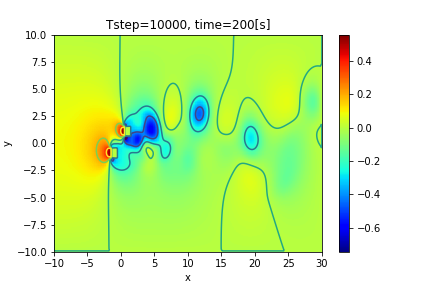
\includegraphics[width=65mm]{object_3.png}
   \caption{$Re=70, u=1.0[m/s]$のとき(角柱2本; 段差あり)}
  \end{center}
  \label{fig:one}
 \end{minipage}
 \begin{minipage}{0.5\hsize}
  \begin{center}
   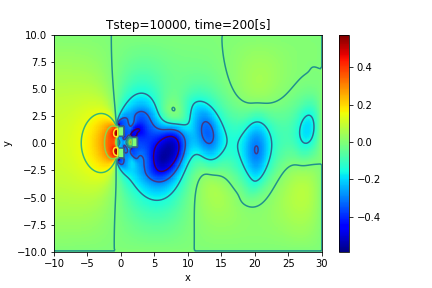
\includegraphics[width=65mm]{object_5.png}
   \caption{$Re=70, u=1.0[m/s]$のとき(角柱3本)}   
  \end{center}
  \label{fig:two}
 \end{minipage}
\end{figure}
\begin{figure}[htbp]
 \begin{minipage}{0.5\hsize}
  \begin{center}
   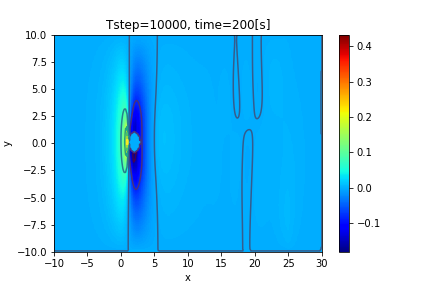
\includegraphics[width=65mm]{object_6.png}
   \caption{$Re=70, u=1.0[m/s]$のとき(円柱)}
  \end{center}
  \label{fig:one}
 \end{minipage}
 \begin{minipage}{0.5\hsize}
  \begin{center}
   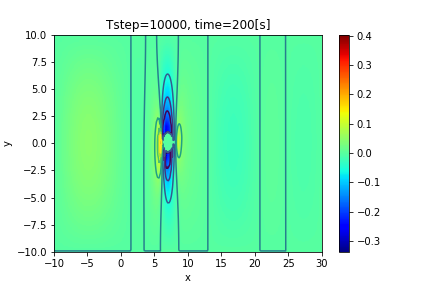
\includegraphics[width=65mm]{object_9.png}
   \caption{$Re=184000, u=0.7[m/s]$のとき(円柱)}   
  \end{center}
  \label{fig:two}
 \end{minipage}
\end{figure}
\begin{figure}[htbp]
\begin{center}
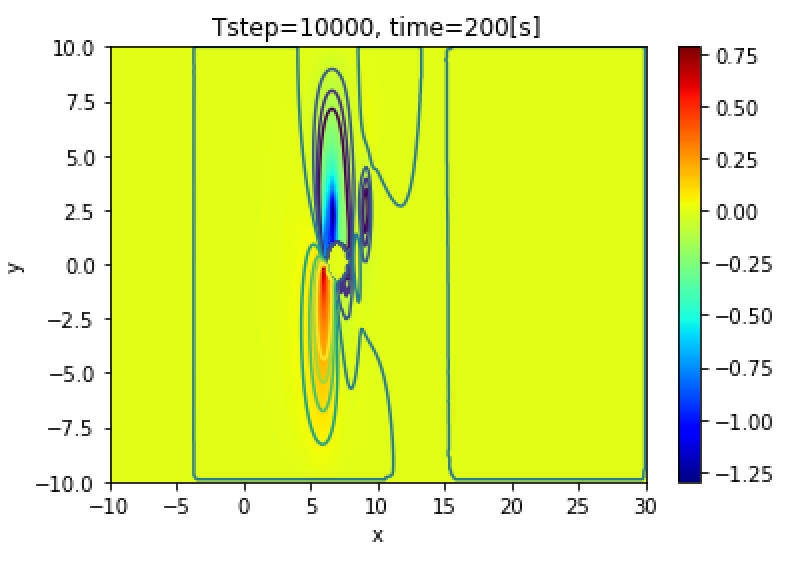
\includegraphics[width=55mm]{object_10.png}
\caption{$Re=184000, u=0.7[m/s], v=0.5[m/s]$のとき(円柱)}
\end{center}
\end{figure}
 \newpage
\section{考察} 
角柱一本の場合, 図1のようにカルマン渦は期待通り観測され, 長く尾を引くように後方に広がっていた. 減衰振動解になっている様子も観測され, 圧力場は左右対称に変化していた. \newline\indent
角柱二本の場合, 角柱の間隔によって後方カルマン渦が出現したりしなかったりしたため個々のカルマン渦の干渉が観測できるような距離に設定した. 角柱付近では圧力場は独立して存在しており, 後方に行くに従って干渉していく. 上半分と下半分での挙動は位相がずれている関係で減衰分を考慮しても明らかに非対称であり, 図2でいうと下が強めあい・上が弱めあいになっている. 減衰の度合いも角柱一本の時より大きい. \newline\indent
角柱三本の場合(並列しても面白くないので後方に配置してみた), 図4のように追加した後ろの角柱の背後に大きな圧力勾配が生じ, 以降急速に減衰している. 図2とは異なり, 図4では上下は独立することなく減衰している; 圧力勾配が大きい分, カルマン渦の発散も早くなっている. なお, 念の為図3で段差ありの角柱2本を試してみたが, この場合は後方の角柱によるカルマン渦のみが生じた. 故に図4も図3二つ分の重ね合わせだと考えることができるかもしれない. \newline\indent
円柱の場合, 水槽実験$^{[1]}$の観測結果と同様にカルマン渦を観測できることが予想されたが, 実験してみた70, 300, 184000のいずれのレイノルズ数においても圧力や速度の振動は観測されず, またカルマン渦も観測することはできなかった(図5参照). そこで円柱付近の格子を細かくすることで, 円柱をより精緻に近似することを目指したがそれでも変わらなかった. 計算機上で同様の問題を発見したという資料$^{[2]}$を見つけたので, これを参考に図6では境界条件による影響を最小限に抑えるため円柱を中心に移動したが, 特に挙動に違いは見られなかった. 図7ではy軸方向の速度場を加え, 場の対称性を崩した. それにより後方の円柱と独立した場所に渦のようなものを観測することができた. 他にもいくつかの条件で試したが, これ以上の渦らしきものを観測することはできなかった.\newline\indent
総じて角柱では容易にカルマン渦を観測することができたが, 円柱では困難であった. 今回は時間等の都合から実行できなかったが, 渦度法などの別のアプローチを用いる必要があると考えられる. 何れにしても, 条件を揃えてもコンピュータシミュレーションと実際の実験で結果が異なってしまうのは興味深かった.
\section{Reference} \noindent
[1] 添付資料「船型試験水槽を用いた円柱のカルマン渦の可視化」レポート \newline
[2] \url{http://www.kochi-tech.ac.jp/library/ron/2000/mec/1010205.pdf}
\end{document}